While we have shown that commuting zone definitions are sensitive to input data and parameters, this sensitivity only matters insofar as it impacts empirical estimates. We demonstrate the consequences of this sensitivity using a well know example of estimates measured at the commuting zone level.

In their paper, \citet{ADH2013} estimate the impact that increased trade competition from China had on manufacturing employment in the United States. To estimate this effect empirically, they use variation in the initial distribution of manufacturing employment at the commuting zone level and national increases in imports from China by manufacturing subsector. Because they use commuting zones as their definition of the local labor market, their empirical analysis is exposed to the critiques we have discussed above.\footnote{We want to acknowledge that Autor, Dorn and Hanson have been incredibly helpful in the process of replicating their paper, both in providing data and helping troubleshoot, as well as being receptive to this exercise.}

Their main estimating equation in the paper is as follows:

\begin{equation}\label{eqn:adh}
\Delta L_{it}^m = \gamma_t + \beta_1 \Delta IPW_{uit} + \beta_2 X_{it} + e_{it}
\end{equation}

Where $\Delta L_{it}^m$ is the decadal change in manufacturing employment in Commuting Zone $i$ following year $t$, $\Delta IPW_{uit}$ is the import exposure measure for the United States, and $X_{it}$ are control variables. All regressions are weighted by population share of the commuting zone.

Since we use slightly different methods of aggregating data, we compare the main estimates from \citet{ADH2013} (Table 1 in their paper) to our replication, which we show in Table \ref{tab:adhreplication}. Each cell in the table is a coefficient from a different regression, and for simplicity we just estimate it for the time period 1990-2000 (other results available upon request). The first column shows the estimates from their paper, while the second column changes the import exposure measures to our replicated measure. In the third column, we use our estimate of the change in manufacturing employment amd weights, rather than the estimate and weights from their data. The final column clusters on commuting zone rather than state.

Overall, the estimates are considerably stable, giving us confidence that we are properly replicating their initial findings. We now turn to demonstrating how these estimates are affected by the concerns with the commuting zone definitions themselves.


% source: name of SAS program
% Last updated:

\begin{table}\centering
\caption{China Syndrome Replication and Comparison, 1990-2000 \label{tab:adhreplication}}
\begin{tabular}{lcccc}
\hline\hline
       & ADH Estimate & Our RHS & Our LHS and Weight & CZ Clustering  \\
       \hline
$\Delta IPW_{cz,t}$ & -0.8875 & -0.8871 & -0.8748 & -0.8748 \\
                   & (0.1812) & (0.1811) & (0.1527) & (0.1243) \\

\hline
\multicolumn{5}{p{6in}}{\footnotesize \textit{Notes}: Table from author's calculations, using data from \citet{ADH2013} and constructed data, based on equation \ref{eqn:adh}. Column 1 is Table 2, Column 1 from ADH (2013). Column 2 replaces their measure of import exposure to ours. Column 3 replaces their measure of change in manufacturing employment and CZ-specific weights with ours. Column 4 does not cluster on state. Standard errors are in parentheses. All coefficients are significant with p-values less than 0.01.}\\
\end{tabular}
\end{table}



\subsection{Effect of Errors in Flows Data}
\FloatBarrier

First, we show how the estimate is affected based on MOE in the commuting flows input data. For this exercise, we used the distribution of margins of error published in the 2009-2013 ACS flows, and matched the ratio based on the flow sizes of the 1990 JTW data.\footnote{These flow size bins are the following percentile bins: 0-50; 50-90; 90-95; 95-99; and 99+.} We then draw from a normal distribution implied by the margins of error, and calculated a new dissimilarity matrix with the perturbed  flows. Using the same cutoff that we used for our replication of TS1996, we produce a new realization of commuting zones, and then repeat the above procedure 1000 times.

\begin{figure}\centering
\caption{Distribution of Effect, 1990-2000 \label{fig:1990dist}}
\begin{tabular}{c}
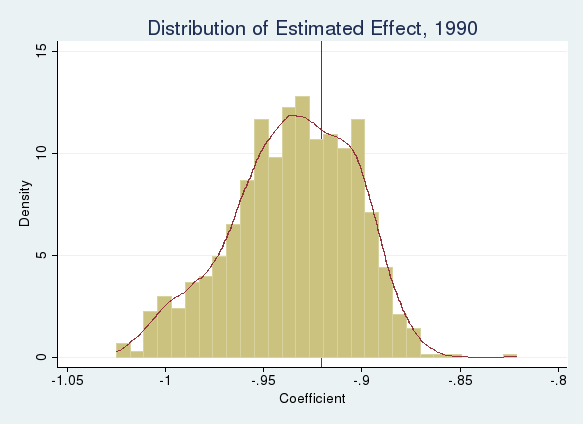
\includegraphics[scale=.5]{./figures/1990_distribution.png}\\
\multicolumn{1}{p{4.5in}}{\footnotesize \emph{Note:} Histogram plots estimates of $\beta_1$ from equation \ref{eqn:adh}, based on commuting zone realizations as outlined in Section \ref{sec:issues}.}
\end{tabular}
\end{figure}

We use these different commuting zone definitions to aggregate counties and then estimate equation \ref{eqn:adh}. These estimates are graphed in Figure \ref{fig:1990dist}, which shows the distribution of the estimated effect for the 1990-2000 period, and the red vertical line shows the estimate under the standard commuting zone defintions. The estimates are somewhat dispersed, with the left tail of the distribution almost 10\% lower than the estimate from ADH; however, the values are within two standard errors of the original estimate. Additionally, the distribution is skewed to the right.

This exercise demonstrates that there is additional uncertainty induced by the construction of the commuting zones that is not addressed in empirical estimates that use these definitions, which may overstate the precision of the results.

%Overall, this underscores the considerable uncertainty in commuting zones, and how this affects empirical estimates in one way. However, there is also ambiguity in how the commuting zones are constructed for reasons separate to the flows. For this discussion we turn to the next subsection.

\subsection{Effects on the Chosen Cutoff}

\begin{figure}\centering
\caption{Differences in Effect Based on Cluster Cutoff \label{fig:cutoff_dist}}
\begin{tabular}{cc}

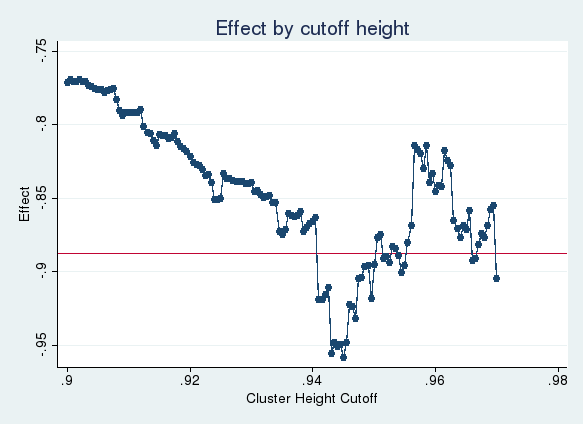
\includegraphics[scale=.4]{./figures/cutoff_1990.png} & 
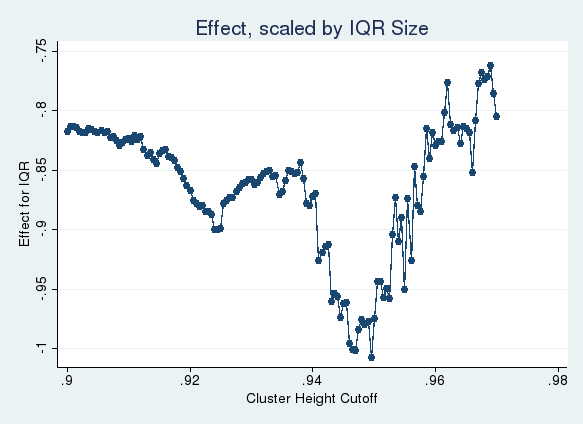
\includegraphics[scale=.4]{./figures/cutoff_iqr_1990.png}\\
(a) Effect by Cutoff Height & (b) Effect by Cutoff Height, Scaled by IQR \\

\multicolumn{2}{p{6.5in}}{\footnotesize \emph{Note:} Author's calculations based on replication of Tolbert and Sizer's method. Panel (a) shows estimates of $\beta_1$ from equation \ref{eqn:adh} for different definitions of commuting zones based on height cutoff, while Panel (b) shows estimates of $\beta_1$ scaled by the difference in exposure between the 25th and 75th percentile commuting zone. The horizontal line in panel (a) is the main estimate from \citet{ADH2013}}
\end{tabular}
\end{figure}

In addition to the uncertainty that is induced by underlying error in the commuting flows, in Section \ref{sec:clusterheight} we showed that the decision of where to stop the clustering process was rather arbitrary, since there is no clear guidance on what cutoff is most appropriate. To demonstrate how the cutoff choice affects the estimate of $\beta_1$ from equation \ref{eqn:adh}, we generate clusters based on cutoffs between 0.9 and 0.97 and estimate the model using the resulting clusters.

Figure \ref{fig:cutoff_dist} displays the results of this exercise, where panel (a) shows the raw coefficient, and panel (b) shows the coefficient scaled by the interquartile range of $\Delta IPW_{uit}$, since this changes depending on the cutoff. In panel (a), the red horizontal line is the estimate from ADH.

Again, our results show that there is some variation in the estimate based on the cutoff value. Around the cutoff value that most closely replicates TS1996, the estimate is the most negative. However, cutoff values marginally higher or lower give different results, which reinforces the point we made with Figure \ref{fig:heightdensity} - the number of clusters that merge is incredibly dense near the cutoff for commuting zones, so that any change in the cutoff changes the commuting zone definitions non-neglibly. This density causes estimates using commuting zone observations to change near the cutoff. Given the sensitivity of estimates to the chosen cutoff, best practices would be to report estimates for a broad range of cutoffs.
